%----------------------------------------------------------------
%
%  File    :  results.tex
%
%  Author :  Wolfgang Radinger-Peer
% 
%  Created :  3. Feb 2019
% 
%  Changed :  3. Feb 2019
% 
%----------------------------------------------------------------


\chapter{\textsc{Results and Discussion}}
\label{chap:results}

\section{Introduction}
\label{sec:introcap4}

Overview of chapter and linking with previous chapter

\section{Visual presentation of the findings}
\label{sec:visualrep}

Findings should be grouped together under relevant headings and discussed accordingly. This means that they should be interpreted and be 
put into the context of previous literature, and findings from other related research. The findings can be presented in a number of ways, 
including tables, graphs, text descriptions and figures. The presentation should be able to communicate the most important aspect of your findings. 
One thing to remember: the figures, tables and graphs should be clearly labelled, numbered and referred to in the text. To achieve a numbering which 
is consistent throughout the thesis you can use captions, and to make it look more professional it is advisable to use the chapter number in the numeration of your visual presentations. 

\section{Tables}
\label{sec:tables}

\section{Usage of tables}
\label{sec:usagetables}

\begin{itemize}
\item The document will be used to look up individual values
\item The document will be used to compare individual values
\item Precise values are required
\item The quantitative information to be communicated involves more than one unit of measures 
\end{itemize}

\section{Example of a good table}
\label{sec:tableexample}


\begin{tabular}{|p{3cm}|p{3cm}|p{3cm}|p{3cm}|p{3cm}|}
	\hline 
	Country of residence & Unique visitors at www.tourism.tallinn.ee/survey & Unique respondents
	& Response rate (%)
	& Partial ratio of unique respondents (\%) \\
    \hline	 
	Finland & 11 & 111 & 111 & 111 \\
	\hline
	Great Britain & 287 & 92 & 32 & 12.0\\
	\hline
	USA & 269 & 85 & 32 & 11.1\\
	\hline
	Germany & 166 &	39 & 23 & 5.1\\
	\hline
	Norway & 166 & 33 & 20 & 4.3\\
	\hline
	Russia & 132 & 29 & 22 & 3.8\\
	\hline
	Sweden & 114 & 47 & 41 & 6.1\\
	\hline
	Italy & 81 & 26 & 32 & 3.4\\
	\hline
	Lithuania & 63 & 23 & 37 & 3.0\\
	\hline
	Latvia & 63 & 27 & 43 & 3.5\\
	\hline
	Spain & 49 & 16 & 33 & 2.1\\
	\hline
	Denmark & 42 & 21 & 50 & 2.7\\
	\hline
	Holland & 39 & 17 & 44 & 2.2\\
	\hline
	France & 37 & 11 & 30 & 1.4\\
	\hline
	Belgium & 30 & 13 & 43 & 1.7\\
	\hline
	Austria & 26 & 16 & 62 & 2.1\\
	\hline
	Poland  & 22 & 4 & 18 & 0.5\\
	\hline
	Japan & 15 & 2 &	13 & 1.3\\
	\hline
	Ireland & 10 & 10 & 100 & 1.3\\
	\hline
	China  & 9 & 2 & 22 & 0.3\\
	\hline
	Other in Europe & 217 & 54 & 25 & 7.0\\
	\hline
	Other outside Europe & 354 & 81 & 23 & 10.5\\
	\hline\hline
	Total: & 2515 & 769  &   &  \\
	\hline 
\end{tabular} 
	
\section{Graphs or figures}
\label{sec:tableexample}

Graphs and figures are used to give a compact overview of material. Indeed, each graph/figure is a component of the paper; however, a chart should be understandable on its own terms. 
For this reason, all abbreviations (apart from the usual statistical abbreviations) must be explained and the unit of measurement stated. 
The presentation of all charts should be consistent throughout, but the way in which you format your tables is up to you. 


\section{Usage of figures}
\label{sec:figures}

\begin{itemize}
\item The message is contained in the shape of the values
\item The document will be used to reveal relationships among multiple values 
\end{itemize}

 
\section{Examples}
\label{sec:figuresExamples}

\begin{figure}[!htb]
        \center{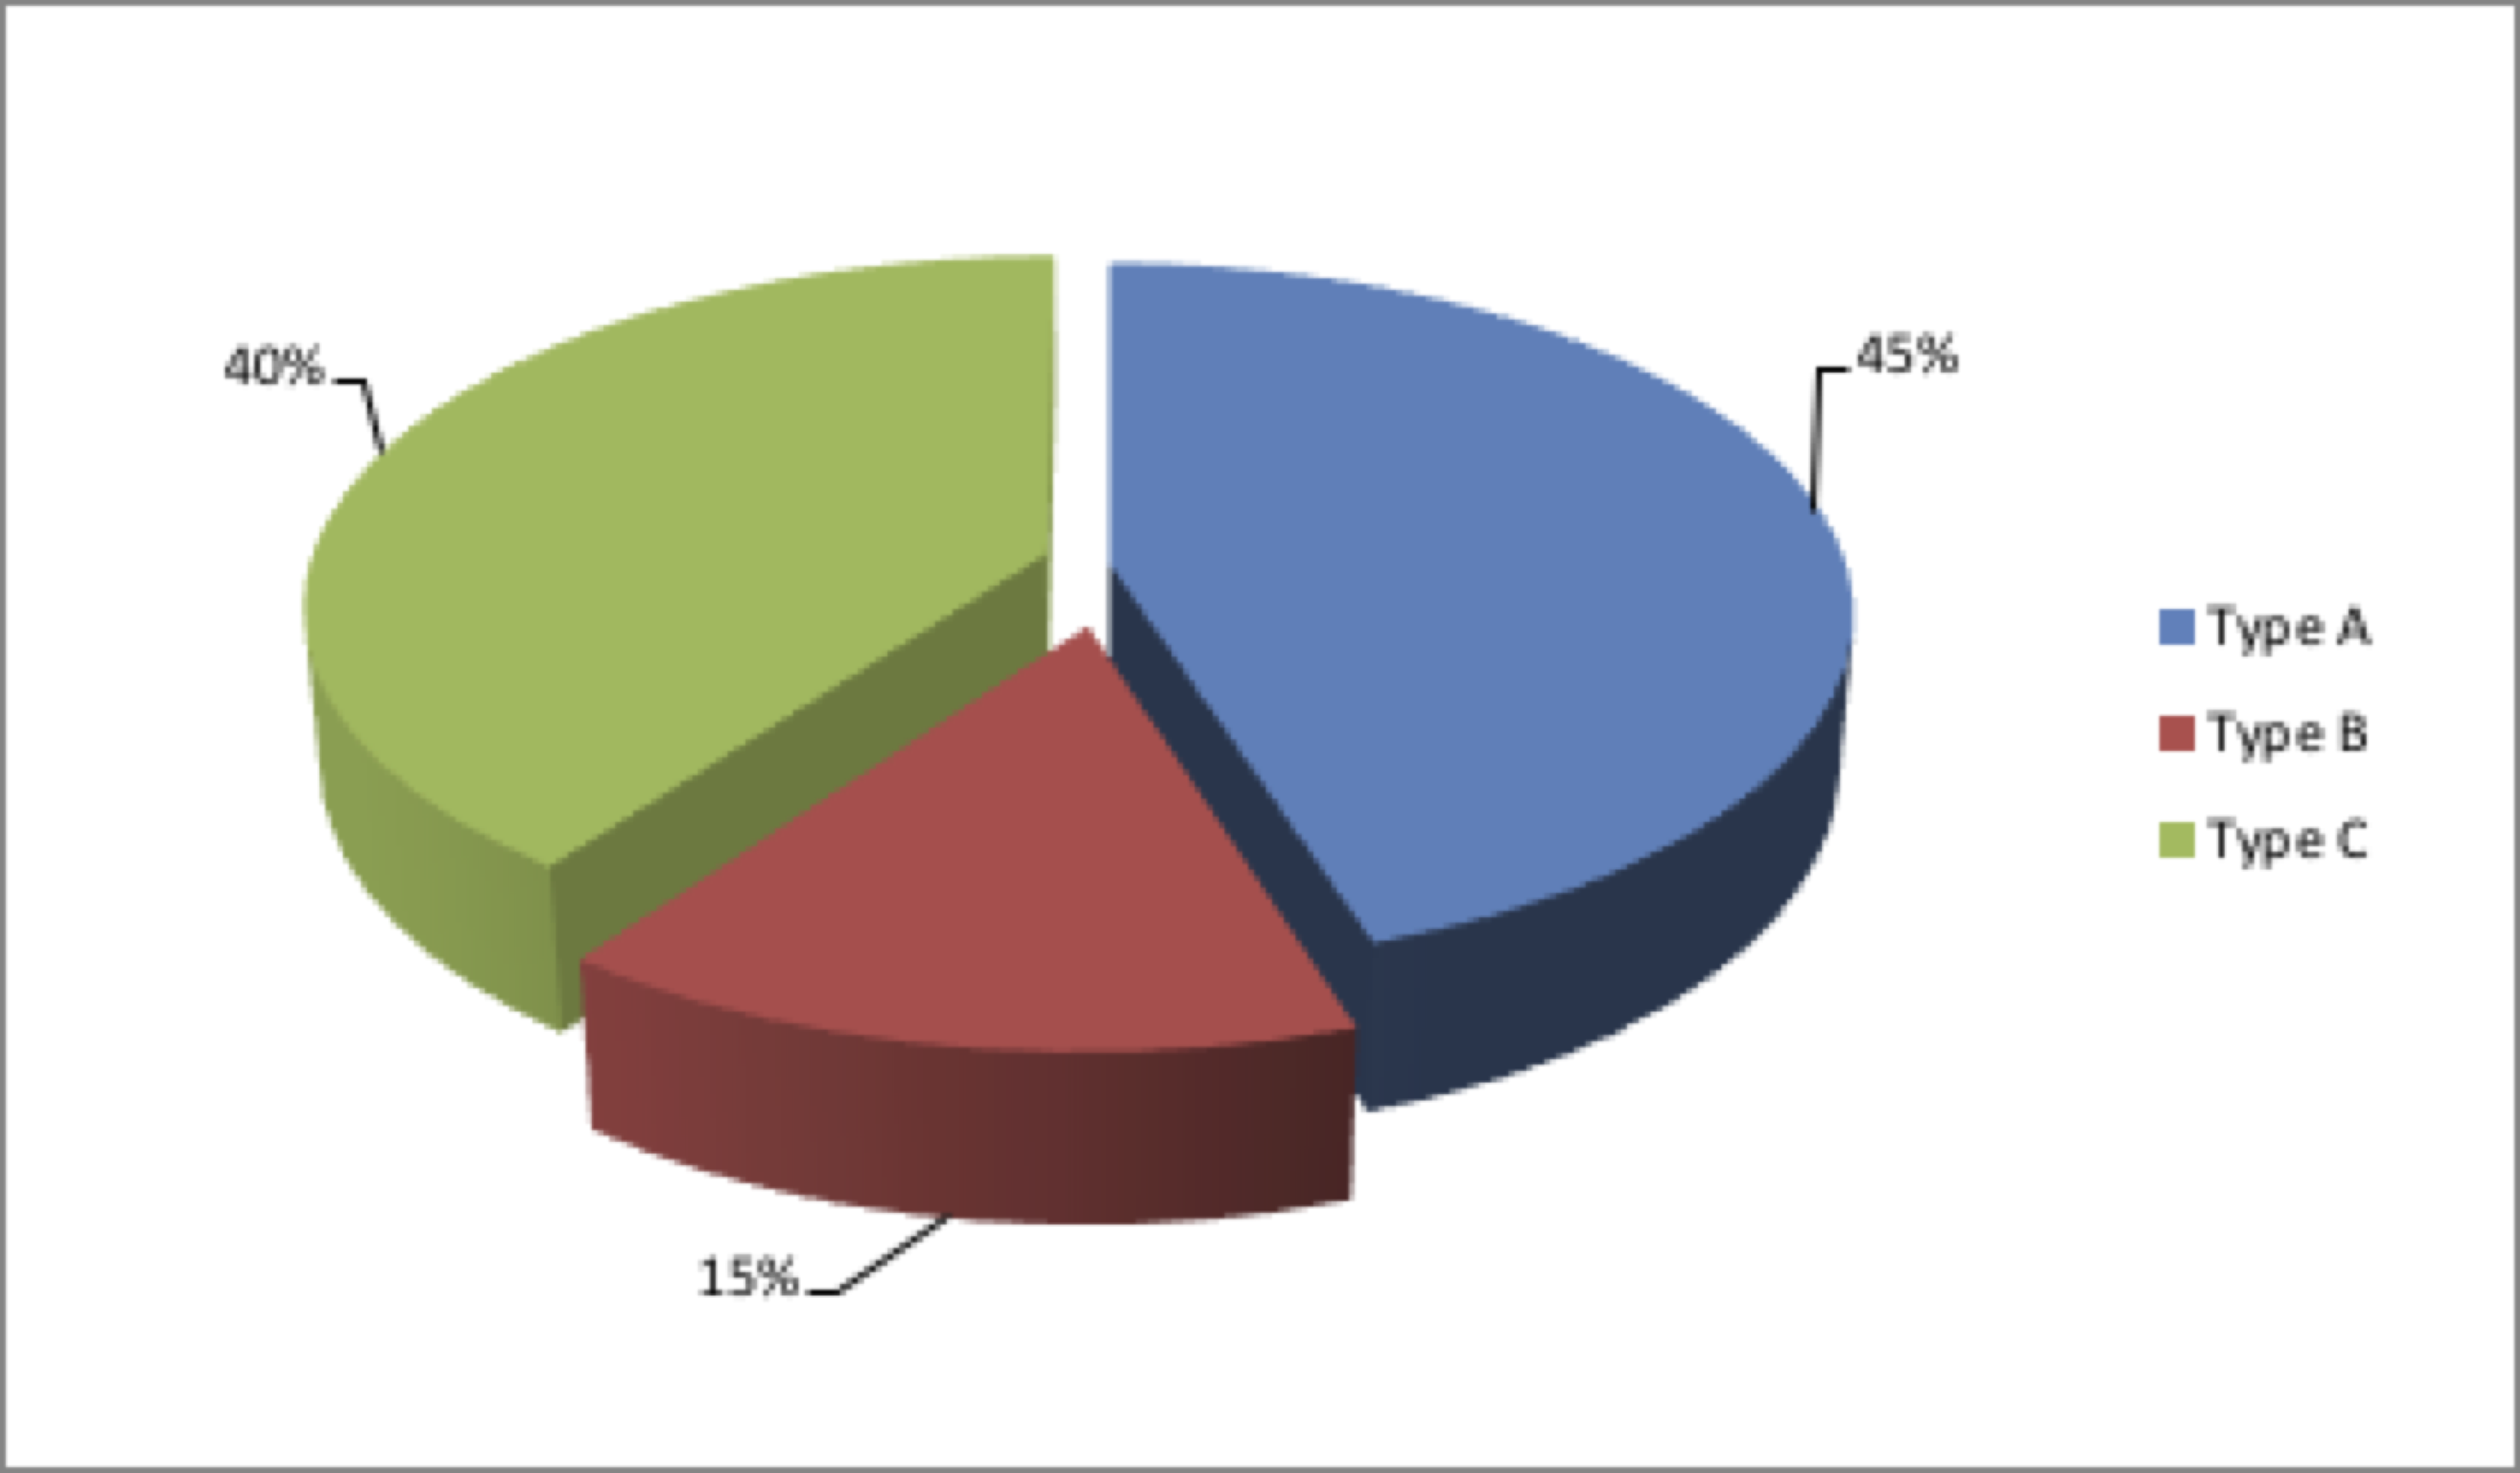
\includegraphics[width=\textwidth]
        {piechart.png}}
       \caption{\label{fig:piechart} EXAMPLE PIE CHART}
\end{figure}

\begin{figure}[!htb]
        \center{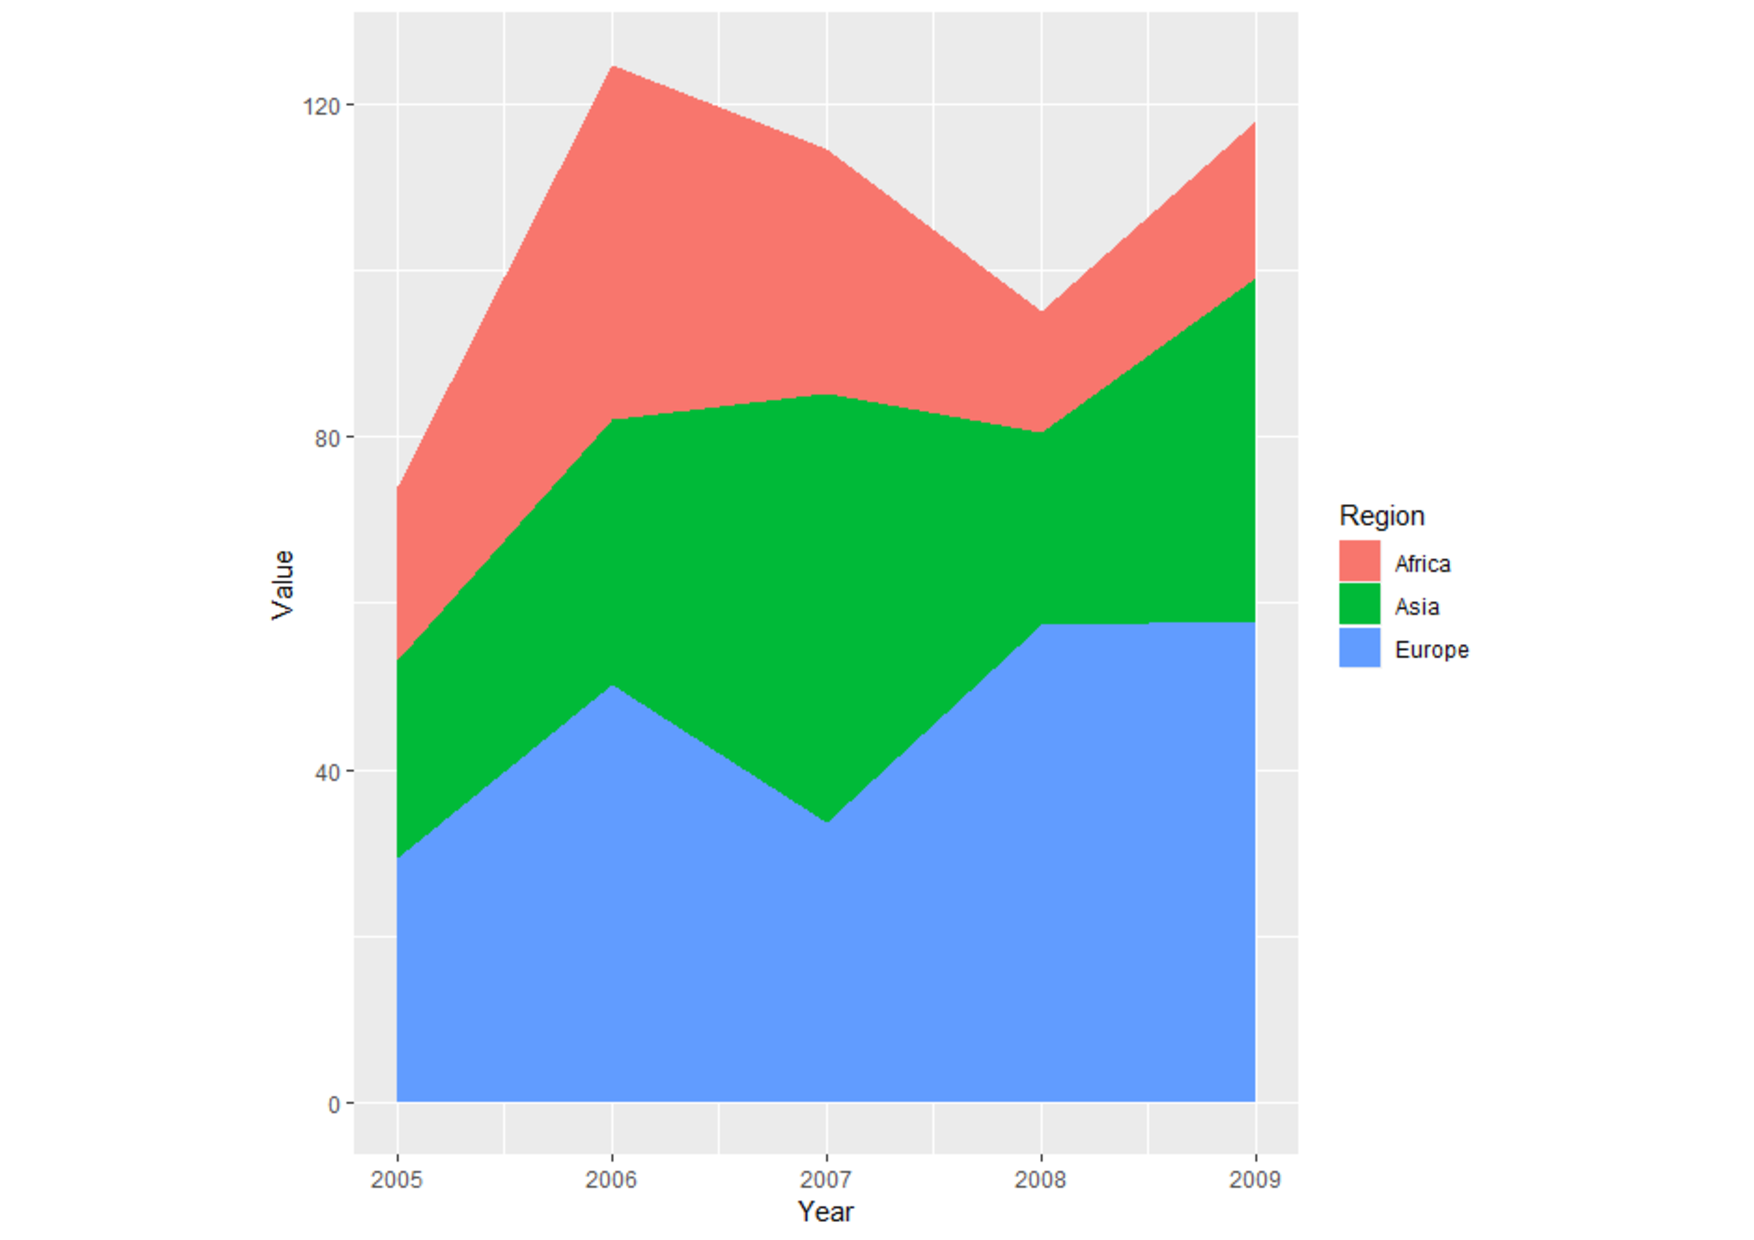
\includegraphics[width=\textwidth]
        {areachart.pdf}}
        \caption{\label{fig:areachart} EXAMPLE AREA CHART}
\end{figure}

\begin{figure}[!htb]
        \center{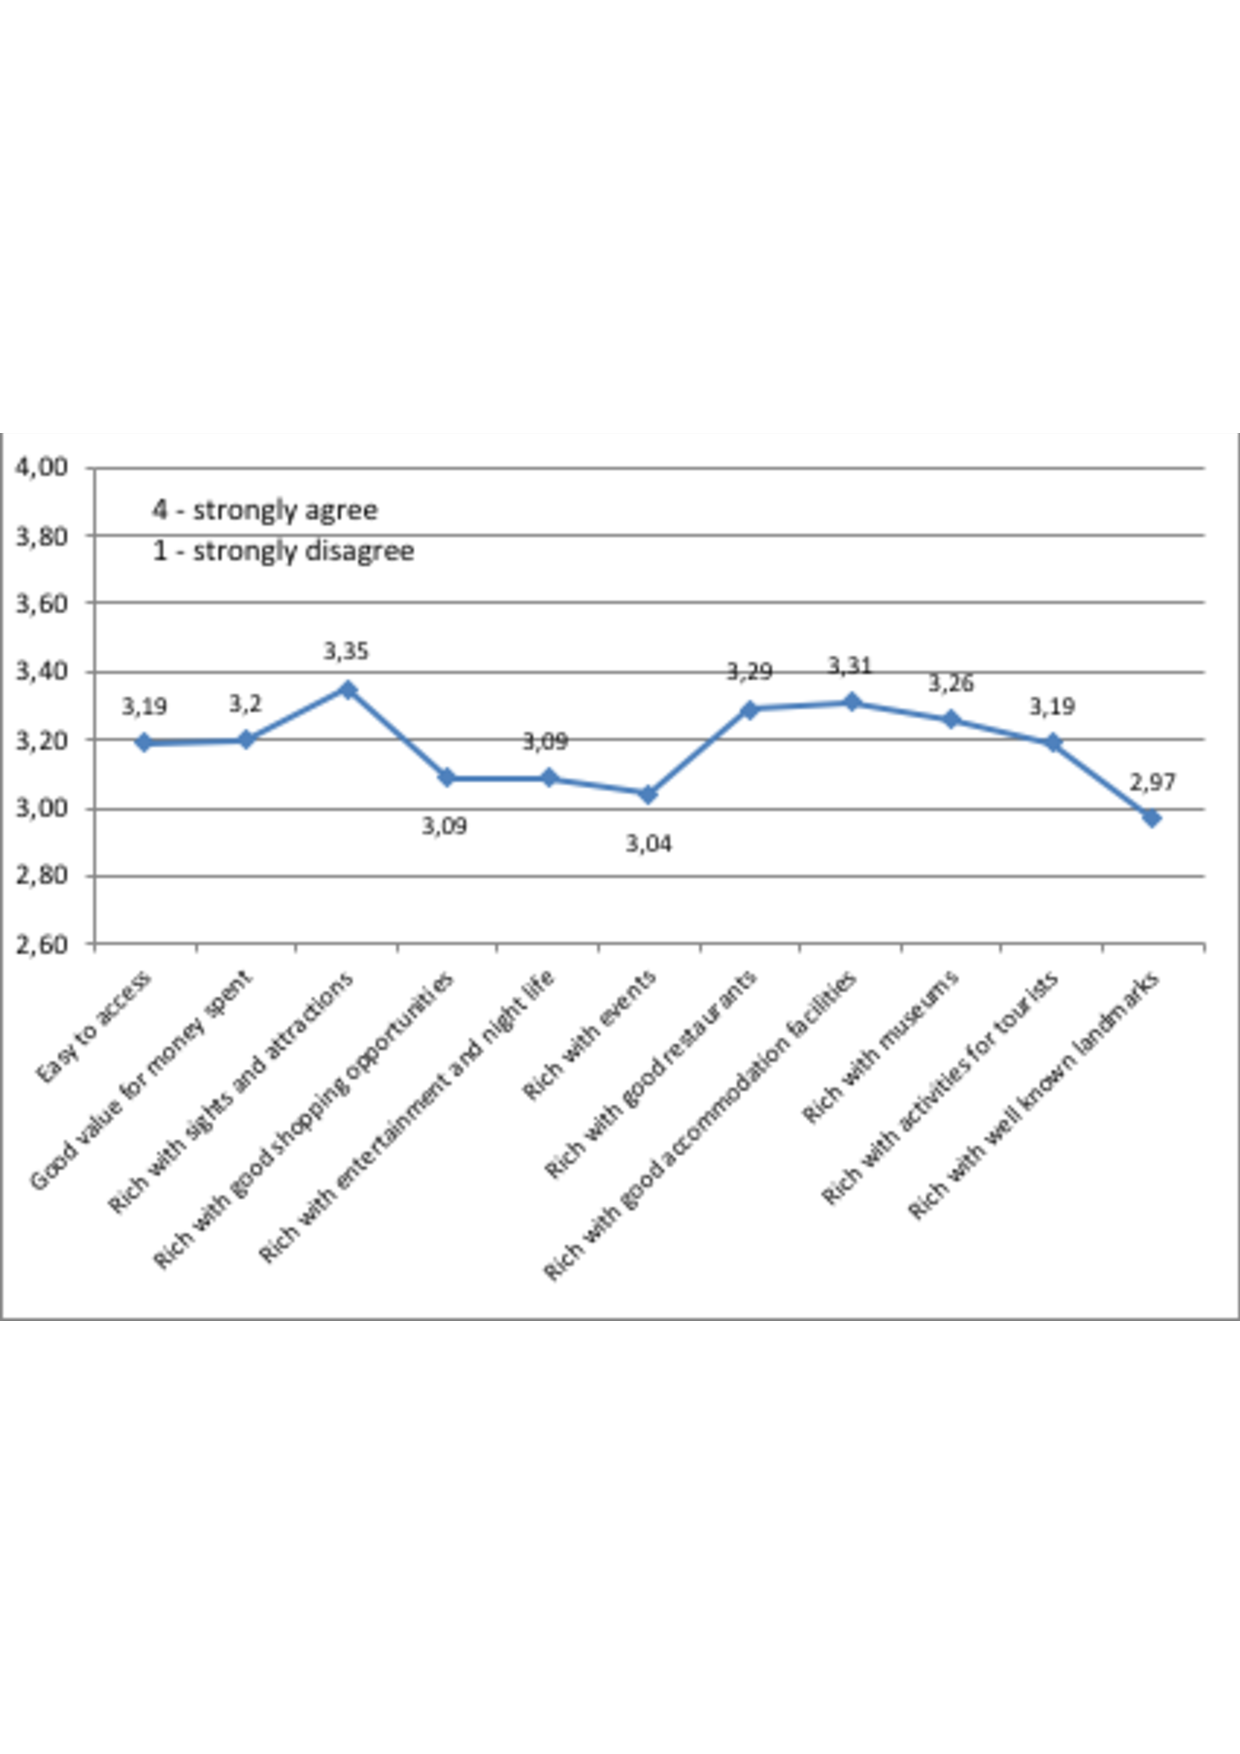
\includegraphics[width=\textwidth]
        {linechart.pdf}}
        \caption{\label{fig:linechart} EVALUATION OF FUNCTIONAL IMAGE ATTRIBUTES, Source: Tsirk, 2009}
\end{figure}      

\section{Qualitative research}
\label{sec:qualitativeresearchs}

This necessitates the use of text description. Although content analysis may produce quantitative results which may be displayed using graphs or tables, quotes from qualitative research are important to support your arguments. 

\subsection{Examples of figures created from content analysis}
 
 \begin{figure}[!htb]
        \center{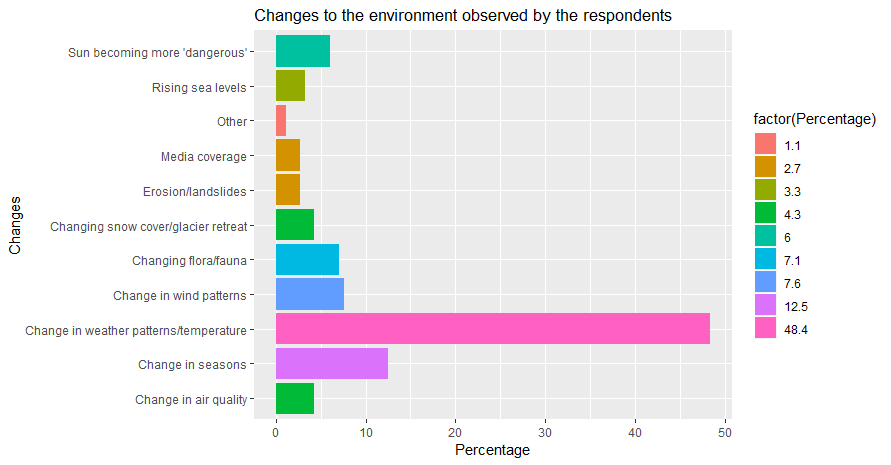
\includegraphics[width=\textwidth]
        {responses.png}}
        \caption{\label{fig:my-label} CHANGES TO THE ENVIRONMENT OBSERVED BY THE RESPONDENTS}
\end{figure}    


\section{Quotations}

“Quotations are statements which have been made explicitly by your respondents.”
“These may be included to highlight specific points that you are making, accompanied by text and interpretation.”

\section{Conclusion}
\label{sec:conclucionchapter4}
Short summary and link to next chapter


